%%%%%%%%%%%%%%%%%%%%%%%%%%%%%%%%%%%%%%%%%%%%%%%%%%%%%%%%%%%%%%%%%%%%%%%%%%%%
% AGUJournalTemplate.tex: this template file is for articles formatted with LaTeX
%
% This file includes commands and instructions
% given in the order necessary to produce a final output that will
% satisfy AGU requirements, including customized APA reference formatting.
%
% You may copy this file and give it your
% article name, and enter your text.
%
%
% Step 1: Set the \documentclass
%
% There are two options for article format:
%
% PLEASE USE THE DRAFT OPTION TO SUBMIT YOUR PAPERS.
% The draft option produces double spaced output.
%

%% To submit your paper:
\documentclass[draft]{agujournal2019}
\usepackage{url} %this package should fix any errors with URLs in refs.
\usepackage{lineno}
\usepackage{color}
\graphicspath{ {figures/} }
\linenumbers
%%%%%%%
% As of 2018 we recommend use of the TrackChanges package to mark revisions.
% The trackchanges package adds five new LaTeX commands:
%
%  \note[editor]{The note}
%  \annote[editor]{Text to annotate}{The note}
%  \add[editor]{Text to add}
%  \remove[editor]{Text to remove}
%  \change[editor]{Text to remove}{Text to add}
%
% complete documentation is here: http://trackchanges.sourceforge.net/
%%%%%%%

\draftfalse

\journalname{JGR: Space Physics}


\begin{document}

\title{Statistical Properties of Electron Curtain Precipitation Derived with AeroCube-6}

%% ------------------------------------------------------------------------ %%
%
%  AUTHORS AND AFFILIATIONS
%
%% ------------------------------------------------------------------------ %%

\authors{M. Shumko\affil{1}, A.T. Johnson\affil{1},  T.P. O'Brien\affil{2}, D.L. Turner\affil{3}, J.G. Sample\affil{1}, J.B. Blake\affil{2}, L.W. Blum\affil{4}, A.J. Halford\affil{4}}


\affiliation{1}{Department of Physics, Montana State University, Bozeman, Montana, USA}
\affiliation{2}{Space Science Applications Laboratory, The Aerospace Corportation, El Segundo, California USA}
\affiliation{3}{Johns Hopkins Applied Physics Laboratory, Laurel, Maryland, USA}
\affiliation{4}{NASA's Goddard Space Flight Center, Greenbelt, Maryland, USA}


\correspondingauthor{M. Shumko}{msshumko@gmail.com}

\begin{keypoints}
\item We used the dual AeroCube-6 CubeSats to identify stationary, narrow, and persistent $>30$ keV precipitation in low Earth orbit
\item 90\% of curtains observed are narrower than 21 kilometers in latitude
\item A few curtains persistently scattered into the atmosphere for at least six seconds
\end{keypoints}


\begin{abstract}
Curtains are stationary, persistent, and narrow in latitude electron precipitation phenomena recently discovered in low Earth orbit over sequential passes of the dual AeroCube-6 CubeSats. Curtains with electron energies $> 30$ keV were stationary over a variety of spacecraft separations, and observed by the follower spacecraft for up to 65 seconds after the leader. This study expands the recent curtain discovery and quantifies statistical properties of 1634 curtains observed over three years. We found that in low Earth orbit, many curtains are narrower than 10 kilometers in latitude and 90\% are less than 21 kilometers wide. We also found that curtains are an outer radiation belt phenomena that are observed in the late morning and midnight magnetic local time, with a higher occurrence rate at midnight. Furthermore curtains are observed more often at lower geomagnetic activity than microbursts.  We compare every statistical result to microbursts to test the hypothesis that curtains are drifting remnants of microbursts. Lastly, we found a few curtains in the bounce loss cone region in the north Atlantic Ocean where particle drift motion is impossible. In one such example, a curtain was continuously scattered for at least six seconds so curtains can be a significant source of $> 30$ keV electrons into the atmosphere.
\end{abstract}

\section{Plain Language Summary}

\section{Introduction}
Curtains are a stationary electron precipitation phenomena observed in low Earth orbit (LEO). They are narrow in latitude and appear stationary for up to a minute between subsequent satellite passes. \citeA{Blake2016} recently discovered curtains with the $> 30$ keV electron dosimeters onboard the dual AeroCube-6 (AC6) CubeSats that operated together between 2014 and 2017. This discovery was possible due to AC6's actively maintained in-track separation between a few hundred meters and a few hundred kilometers. Besides the \citeA{Blake2016} discovery study not much is known about curtains including what they are, how are they generated, their statistical properties, and their impact on the atmosphere. Answering these questions is an essential next step towards a more complete understanding of how curtains, and particle precipitation in general, affect the magnetosphere and Earth.

In low Earth orbit (LEO) curtains are narrower than a few tens of kilometers in latitude so a LEO satellite, such as AC6, will pass through them in a second or less. Curtains appear spiky in the electron data. AC6 also observes similar-looking transient precipitation called electron microbursts. Both microbursts and curtains appear appear spiky in the AC6 data for different reasons: microbursts primarily for being temporally short, and curtains primarily for being narrow in latitude. Hence AC6, and other recently developed multi-spacecraft missions, are necessary to identify and distinguish between curtains and microbursts.

Microbursts have been observed since mid 1960s by high altitude balloons and satellites and are also a spiky increase of electrons shorter than a second but are not spatially stationary \cite<e.g.>{Anderson1964, Lorentzen2001a, O'Brien2003, Douma2017}. The  companion study to this work by \citeA{Shumko2020} calculated the spatial size of microbursts using simultaneous observations of microbursts observe by AC6. The impact of microbursts on the environment is substantial. \citeA{Lorentzen2001b}, \citeA{Thorne2005}, \citeA{Breneman2017}, and \citeA{Douma2019}---among others---estimated that microbursts can deplete the outer radiation belt electrons in about a day. Furthermore, \citeA{Seppala2018} modeled a 6 hour microburst storm and concluded that microbursts depleted mesospheric ozone by roughly 10\%. Thus, it is important to understand the connection, if any, between microbursts and curtains. Curtains and microbursts can be easily misidentified from a single spacecraft so we need to reevaluate single-satellite microburst studies. If curtains are numerous then the estimated microburst occurrence rates are overestimated. Furthermore, the microburst impact on the atmosphere and the outer radiation belt is overestimated.

\citeA{Blake2016} proposed the following hypothesis that explains the curtain-microburst relationship. If a microburst is not completely lost in the atmosphere after the initial scatter, the remaining microburst electrons will spread out (bounce phase disperse) along the entire magnetic field line over a few bounce periods. Concurrently these electrons drift to the east, with higher energy electrons drifting at a faster rate. Therefore, if this hypothesis is true, the initially localized microburst is spread out in longitude into the shape of a curtain. The idea of curtains is not entirely new, and \citeA{Lehtinen2000} presented a different hypothesis that curtains can be created by energetic runaway beams driven by lightning.

This study expands the \citeA{Blake2016} study by estimating statistical properties of curtains. We use 1634 confirmed curtain observations to study the distributions of: the curtain width in latitude, the geomagnetic conditions favorable to curtains, and curtain distribution in L and magnetic local time (MLT). Lastly we will address the hypothesis that curtains are drifting remnants of microbursts by showing examples of curtains observed in the BLC region.

\section{Instrumentation} \label{instrumentation}
The AC6 mission was a pair of 0.5U (10x10x5 cm) CubeSats built by The Aerospace Corporation designed to measure the electron and proton environment in low Earth orbit \cite{O'brien2016}. AC6 was launched on 19 June 2014 into a 620x700 km, $98^\circ$ inclination orbit. The AC6 orbit over the three year mission lifetime was roughly dawn-dusk, and precessed only a few hours in MLT; 8-12 MLT in dawn and 20-24 MLT in dusk. The two AC6 spacecraft, designated as AC6-A and AC6-B, separated after launch and were in proximity for the duration of the three year mission---maintained by an active attitude control system. The attitude control system allowed them to precisely control the amount of atmospheric drag experienced by each AC6 unit using the surface area of their solar panel ``wings". By changing their orientation, AC6 was able to maintain a separation between 2-800 km, confirmed with the Global Positioning System. The two AC6 units were in a string of pearls configuration so one unit, typically unit A, was leading the other by an in-track lag---the time it would take the following spacecraft to catch up to the position of the leading spacecraft. To convert between the AC6 in-track separation and in-track lag, we use a typical 7.5 km/s LEO velocity. The in-track lag was readily available with the Global Positioning System which makes it easy to study precipitation phenomena observed at the same time, and at the same position by shifting one time series by the in-track lag.

Each AC6 unit contains three Aerospace microdosimeters (licensed to Teledyne Microelectronics, Inc) that measure the electron and proton dose in orbit \cite{O'brien2016}. The dosimeter used for this study is dos1 with a $30$ keV electron threshold. dos1 is used for this study because the other dosimeters either responded primarily to protons or were not identical between unit A and B. All dosimeters sample at 1 Hz in survey mode, and 10 Hz in burst mode. 10 Hz data was readily available from both AC6 units from June 2014 to May 2017 while their in-track lag was less than 65 seconds, and at times was a fraction of a second. Figure \ref{a_10Hz_dist} shows the distribution of 10 Hz data as a function of AC6 in-track lag. The variety of AC6 separations and data availability over the three-year mission makes it possible to study tranisent electron microburst precipitation \cite{Shumko2020} and now stationary electron curtain precipitation.

\section{Methodology} 
\subsection{Curtain Identification} \label{curtain_identification}
The 10 Hz data was used to identify curtains with the following two criteria that are described below: a high spatial correlation, and spiky. Before we applied the identification criteria, the AC6-B time series was shifted by the in-track lag to spatially align it with the AC6-A time series. 

The first identification criterion is a 1-second rolling Pearson correlation applied to both time series. Spatial features with a correlation greater than 0.8 are considered highly correlated. The second criterion is applied to any features determined to be highly correlated to check if they are also spiky. Similar to how precipitation bands were identified by \citeA{Blum2015} and microbursts by \citeA{Greeley2019}, we find spiky precipitation by quantifying the number of Poisson standard deviations, $\sigma$, that a dos1 count rate is above a 10-second centered running average, $B_{10}$. Locations where dos1 is at least two $\sigma$ above $B_{10}$, in other words $dos1 > 2\sqrt{B_{10}} + B_{10}$, are considered spiky. 

We tuned the detection parameters to identify many candidate curtains while being feasible to check every detection. One author visually inspected 6149 candidate curtains and 1634 quality curtains were confirmed. Four curtain examples are shown in Fig. \ref{fig1}. In each example, the unmodified time series is shown in the top row and the spatially-aligned time series the bottom row. The in-track lag used to shift the bottom row is annotated by $dt$, corresponding to an AC6 in-track separation annotated by $s$. The bottom row shows curtains observed at the same location that were correlated for at least 3 to 26 seconds.

\begin{figure}
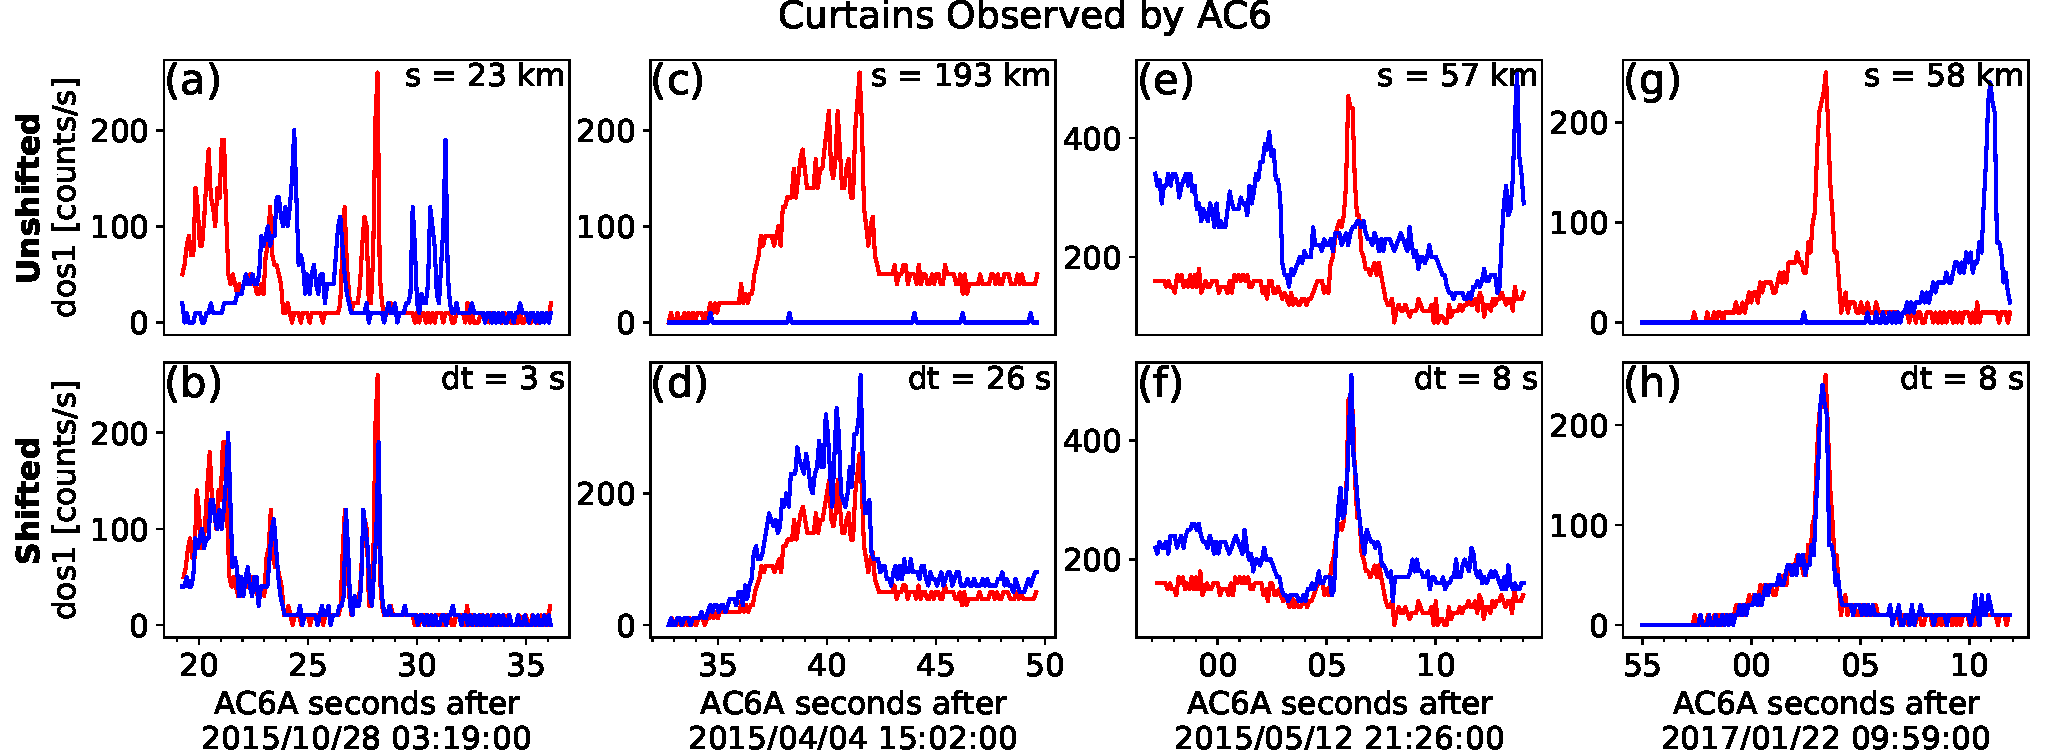
\includegraphics[width=\textwidth]{fig1.pdf}
\caption{Four examples showing the AC6 $> 30$ keV electron data taken by AC6 at the same time in the top row and at the same position in the bottom row. AC6-A, whose data is shown with red curves, was $s$ kilometers ahead of AC6-B. To show the data at the same position the AC6B time series was shifted by the in-track lag annotated by dt. These examples show that curtain precipitation was highly correlated for up to 26 seconds.}
\label{fig1}
\end{figure}

\subsection{Differentiating Between Drifting and Precipitating Curtains}

The AC6 dosimeters lack the necessary pitch angle resolution to differentiate between drifting and precipitating electrons to test the \citeA{Blake2016} hypothesis. One common method of distinguishing between precipitating, drifting, and trapped particles is using particle measurements in conjunction with the location of the South Atlantic Anomaly (SAA).

Earth's magnetic field is asymmetric which creates a region of weaker magnetic field in the South Atlantic Ocean called the South Atlantic Anomaly. 
While some particles observed in LEO are trapped and will execute closed drift paths, most particles observed in LEO are quasi-trapped: they drift around the Earth until they reach the SAA. Within the SAA, the weaker magnetic field strength can lower the electron's mirror point altitude into the atmosphere, where collisions with the atmospheric ions are more numerous and the particle is lost. 

Particles that have pitch angles in the drift loss cone will precipitate within one drift period (often within the SAA). Particles with smaller equatorial pitch angles (less than about $10^\circ$) that are lost in the atmosphere within one bounce are in the bounce loss cone. Traditionally, we define a particle with a mirror point altitude at or below 100 km to be in the BLC.

In most regions outside of the SAA and its conjugate point, AC6 will observe electrons in both the drift and bounce loss cones. In the SAA, AC6 does not only observe particles that are immediately lost, but a combination of particles that are in the drift loss cone, bounce loss cone, and trapped (the trapped particles that locally mirror at AC6's altitude in SAA will mirror higher everywhere else). In the region magnetically conjugate to the SAA in the North Atlantic, AC6 only observes particles in the BLC. \textcolor{red}{which version A or B? A: A particle that is observed by AC6 either precipitates locally or mirrors at or below AC6. If a particle mirrors at or below AC6, the particle will bounce towards its conjugate mirror point deep in the atmosphere in the SAA. \newline B: If an electron makes it to AC6's altitude, it might be in the local loss cone and precipitate in the local hemisphere. Alternatively, the electron will mirror at or below AC6 and gyrate to the conjugate mirror point in the SAA where the mirror point is deep in the atmosphere or below sea level.} Therefore, any precipitation observed in this region must rapidly precipitate. 

We estimated the BLC region for locally-mirroring electrons in the North Atlantic Ocean using the IRBEM-Lib magnetic field library and the Olson-Pfitzer magnetic field model \cite{irbem, Olson1982}. We defined a latitude-longitude grid spanning the North Atlantic at 700 kilometer altitude (a typical altitude for AC6), and estimated the local magnetic field strength. For each latitude-longitude point we traced the magnetic field line to the southern hemisphere and found the conjugate mirror point altitude. If the conjugate mirror point is at or below 100 kilometers, the particle is likely lost and the assosiated grid point is considered to be in the BLC. Furthermore, a more rigorous bounce loss cone criterion would be if the conjugate mirror point altitude is below sea level. In this case, the electron is definitely lost. Since AC6 can measure locally-mirroring electrons in the North Atlantic, the spacecraft altitude estimates the upper bound mirror point of this population. The BLC region estimated by this method closely matches the BLC region shown in \citeA[Figure 1]{Comess2013} and \citeA[Figure 3]{Dietrich2010}. Furthermore, we repeated the same analysis using the Tsyganenko 1989 model \cite{Tsyganenko1989}, \textcolor{red}{which} yielded similar boundaries.

\section{Results} \label{results}
In the spirit of brevity, we limited the scope of this statistical study to answer three questions:

\begin{enumerate}
\item What is the curtain width in latitude?
\item When and where are curtains observed?
\item Are curtains drifting or locally precipitating?
\end{enumerate} For each of these questions we will compare the curtain distribution with the $>30$ keV microburst distribution from \citeA{Shumko2020}.

\subsection{Curtain Width}
We quantified curtain width in time as the width at half of the curtain's topographic prominence: the height of the peak above the lowest contour that encircles the peak but contains no higher peak. \textcolor{red}{Include a figure? I am hesitant because an illustration of topographic prominence is one Google search away...} The spatial width of a curtain is the product of the observed width in time and the 7.5 km/s orbital velocity. The curtain width is measured along AC6's orbit track that is mostly in latitude, therefore these widths are approximately the curtain width in latitude. The distribution of curtain widths is shown in Fig. \ref{width_dist} by the thick black curve. Curtains are very narrow in latitude. Many curtains are less than 10 km wide, and 90\% are narrower than 21 km.
	
We compared the curtain width distribution to the microburst size distribution estimated in \citeA{Shumko2020}. \citeA{Shumko2020} estimated the microburst size distribution by finding microbursts that were observed simultaneously by both AC6 units so the microburst size must be larger than the AC6 separation. The red curve in Fig. \ref{width_dist} shows the microburst distribution estimated from the ratio of the number of concurrent and nonconcurrent microbursts observed in each separation bin. 

\subsection{When and Where Are Curtains Observed}
The distribution of curtains in L and MLT is shown in Fig. \ref{l_mlt_dist}. Figure \ref{l_mlt_dist}a shows the distribution of the observed curtains and Fig. \ref{l_mlt_dist}b shows the same distribution normalized by the number of quality 10 Hz samples AC6 took in each L-MLT bin. This normalization is shown in Fig. \ref{l_mlt_dist}c. The white bins in the early morning and evening MLT regions in Fig. \ref{l_mlt_dist}a had no observed curtains because the AC6 orbit did not sample there as confirmed by Fig. \ref{l_mlt_dist}c. The normalized curtain distribution in Fig. \ref{l_mlt_dist}b shows an enhanced curtain occurrence in the outer radiation belt in late morning and midnight MLT regions.

Now we quantify the geomagnetic conditions favorable for curtains. Figure \ref{ae_dist} shows the distribution of the Auroral Electroject (AE) index between 2014 and 2017 in solid black. The distribution of the AE index when curtains were observed is shown by the dotted blue lines. Lastly, the distribution of the AE index when $> 30$ keV microbursts were observed is shown with a dashed green lines. 

\begin{figure}
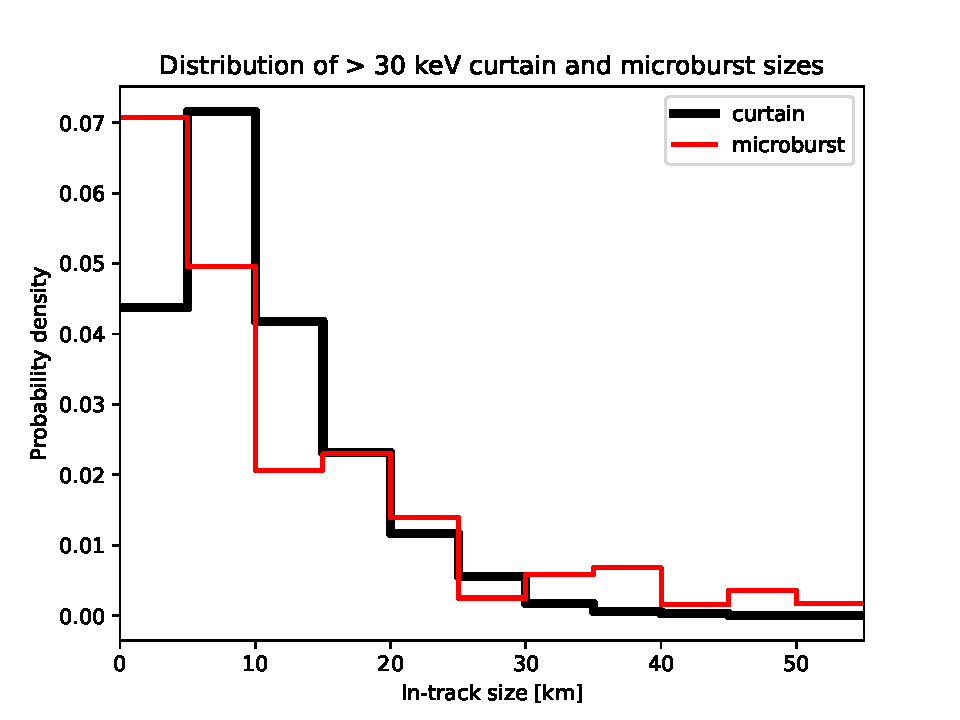
\includegraphics[width=\textwidth]{ac6_curtain_microburst_width_dist.pdf}
\caption{Distribution of curtain width in latitude shown in black and sizes of microbursts when they were simultaneously observed by AC6 is shown in red. Microburst distribution adopted from \citeA{Shumko2020}. The error bars represent the Poisson standard error.}
\label{width_dist}
\end{figure}

\begin{figure}
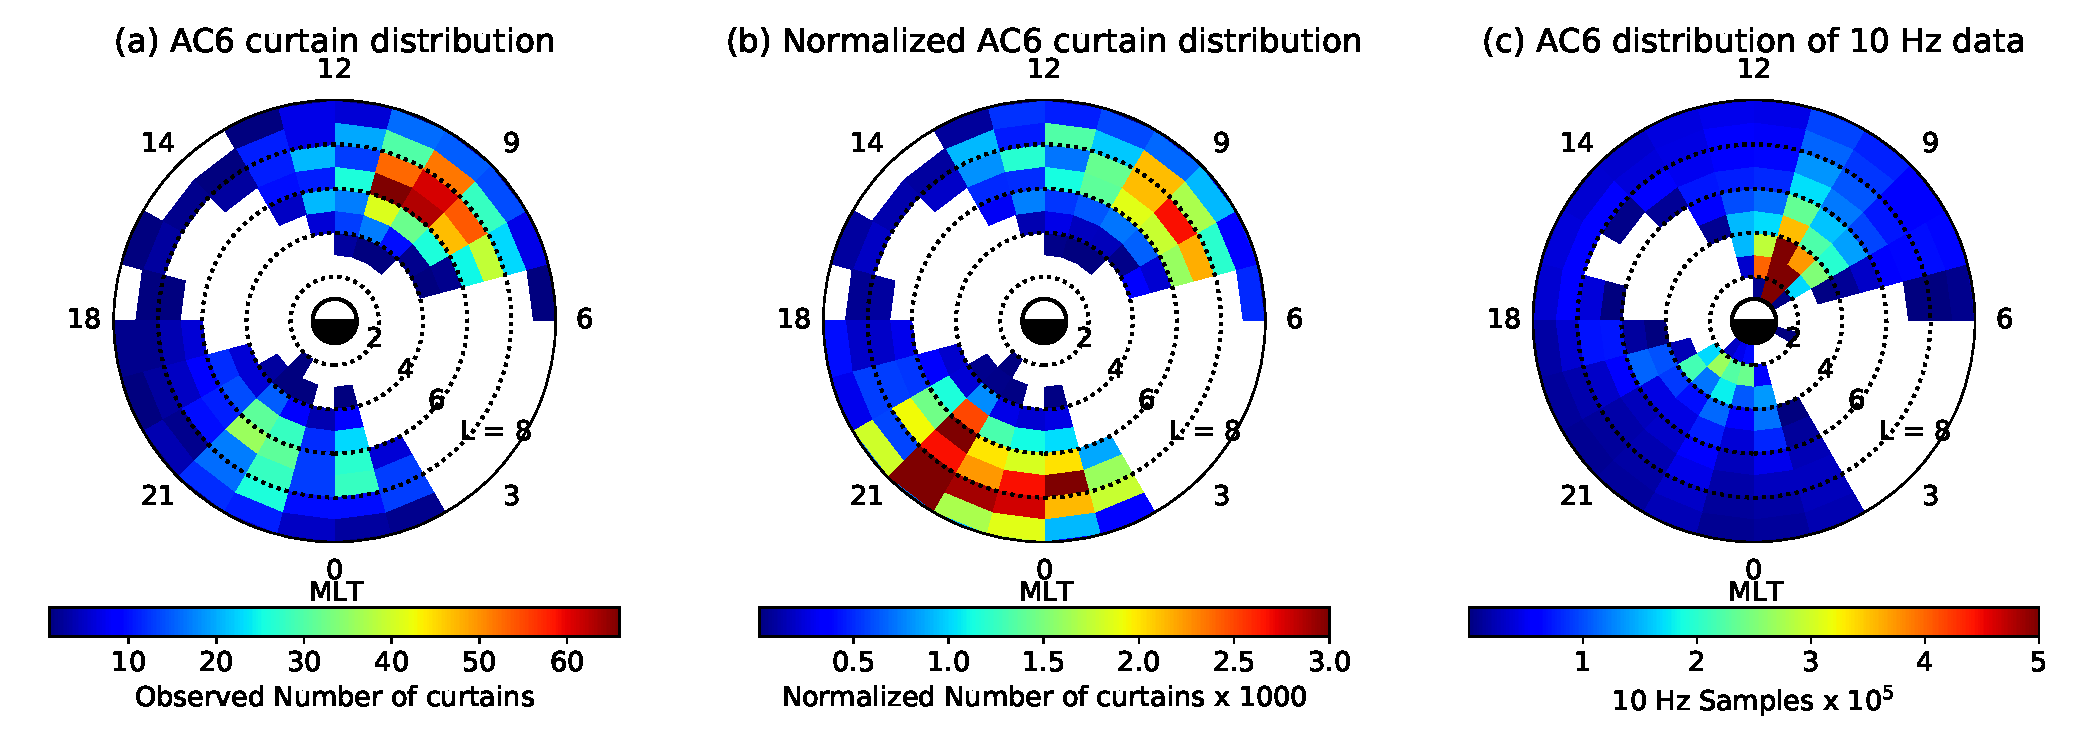
\includegraphics[width=\textwidth]{fig2_2.pdf}
\caption{Distribution of observed curtains by L shell and MLT. Panel a shows the locations of all curtains used in this study. Panel b shows the curtain distribution normalized by the number of quality 10 Hz samples taken in each bin, shown in panel c. The white bins in panels a and b have no observed curtains. In panel c the white bins show where AC6 did not take any 10 Hz data due to its orbit.}
\label{l_mlt_dist}
\end{figure}

\begin{figure}
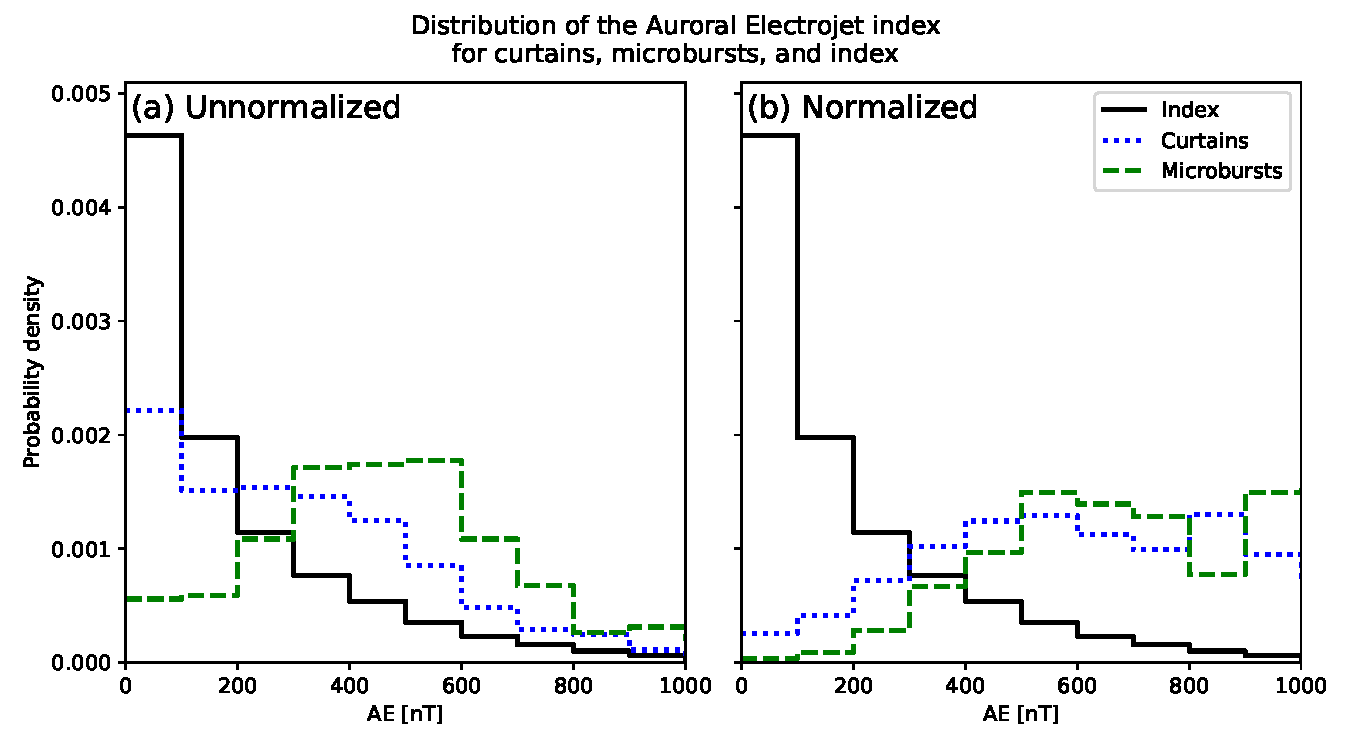
\includegraphics[width=\textwidth]{ac6_curtain_microburst_AE_dist.pdf}
\caption{The distribution of the Auroral Electroject (AE) index from 2014 to 2017. The black curve shows the distribution for the entire 2014-2017 AE data set, the dotted blue curve shows the AE distribution for curtains, and the dashed green curve shows AE the distribution for microbursts studied in \citeA{Shumko2020}. \textcolor{red}{Make a normalized version of this plot}}
\label{ae_dist}
\end{figure}

\subsection{Local Atmospheric Precipitation}
\textcolor{red}{The evidence presented so far hint at, but not directly confirm that, curtains are connected to microbursts. But a few curtains observed in the bounce loss cone put the hypothesis into question.}

Figure \ref{fig3}a shows a map of the northern BLC region in the North Atlantic. The solid blue line is the northern boundary where an electron that mirrors at 700 km locally will mirror at 100 km in the SAA. Immediately south of the solid blue line, the SAA mirror altitude rapidly decreases towards, and below, sea level. The dashed blue line is the boundary where the SAA mirror point altitude is at sea level. South of this line the mirror point is inside Earth. For reference, AC6 takes about 30 seconds to move between the solid and dashed blue curves. The two dotted black curves in Fig. \ref{fig3}a are roughly the boundary of the outer radiation belt, defined as $\mathrm{L}=4-8$.

We found 36 curtains that were observed inside the BLC region. Figure \ref{fig3}b-e shows 4 examples with time-shifted series plots, along with the AC6 in-track lag, L and MLT during the observations annotated. The AC6 locations where these curtains were observed are shown in Fig. \ref{fig3}a with red stars and the corresponding panel labels.

\begin{figure}
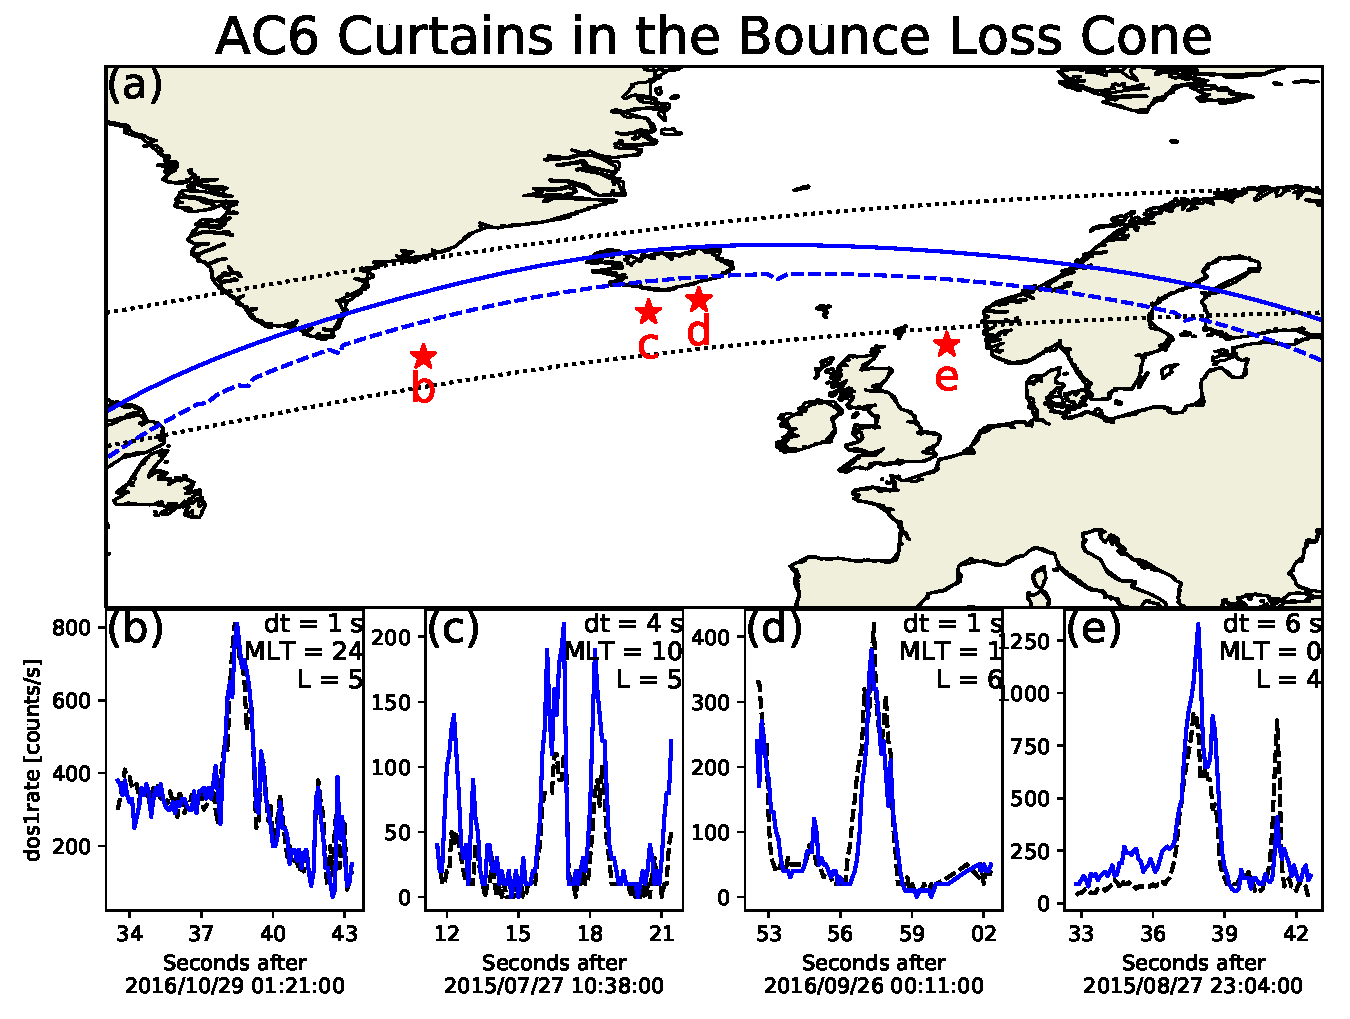
\includegraphics[width=\textwidth]{fig3.pdf}
\caption{Curtains observed inside the bounce loss cone region. Panel a shows a map of the North Atlantic region with the outer radiation belt, defined by an L shell range between 4 and 8, shown with the dotted black curves. The solid blue curve shows the northern boundary of the bounce loss cone region. Along this curve, electrons observed at a 700 kilometer altitude in the North Atlantic will mirror at 100 kilometers in the SAA. A more strict bounce loss cone criteria is the dashed blue curve that represents a mirror point altitude at sea level in the SAA. The 4 red stars with labels show the locations of the curtain examples shown in panels b-e. The panels b-e show the 4 example curtains with the AC6-A shown by the red line, and AC6-B with the blue line. AC6-A was ahead in all examples except panel d.}
\label{fig3}
\end{figure}

\section{Discussion} \label{discussion}
\subsection{Curtain Width In Latitude}
Curtains are very narrow in latitude. Figure \ref{width_dist} shows the width in latitude of many curtains are on the order of 10 kilometers and 90\% are narrower than 21 km. Scaled to the magnetic equator, where we presume curtains are generated, these latitudinal widths correspond to a source with a radial scale size of a few hundred kilometers. As shown in Fig. \ref{fig1}f and \ref{fig1}h; it is remarkable that some curtains maintain a fine structure after multiple seconds with little observable difference. Sometimes curtains appear to be slightly and systematically shifted in latitude, while maintaining their shape (not shown).

If curtains are remnants of microbursts then the distribution of curtain widths in latitude correspond to the microburst size distribution. Figure \ref{width_dist} shows a good correspondence between the distribution of curtain widths in latitude and the microburst size distribution from \citeA{Shumko2020}. Therefore, it is reasonable to believe that curtains and microbursts are related, but this result needs to be closely inspected for sources of bias. 

The microburst scale size distribution, as described in \citeA{Shumko2020}, is the fraction of microbursts observed simultaneously to all microbursts observed either simultaneously or by only one AC6 unit. A microburst observed simultaneously must be larger than the spacecraft separation so the microburst distribution represents a lower bound. \citeA{Shumko2020} attempted to account for this bias but it is difficult. This bias that shifts the microburst distribution to smaller sizes so in the microburst size distribution shown in Fig. \ref{width_dist} is underestimated.

Furthermore the detection algorithm described in section \ref{curtain_identification} has a width bias. For wide curtains with a similar width to the detection algorithm's 10-second baseline, the 10-second baseline is then calculated using the enhanced curtain counts instead of the background and is increased above the true background and thus the curtain peak is less pronounced relative to the baseline. As a result, the curtain detection algorithm is less sensitive to wider curtains. The result of this bias is similar to the bias inherent in the microburst distribution---the curtain widths are underestimated.

Both of these biases underestimate the true size of curtains and microbursts, so this evidence agrees with the \citeA{Blake2016} microburst-curtain hypothesis.

\subsection{When and Where Are Curtains Observed}
Figure \ref{l_mlt_dist} shows that curtain phenomena originates in the outer radiation belt, and observed relatively more in the evening than morning regions. Unfortunately, the limited AC6 coverage prevents a complete curtain distribution in MLT. From the MLT information we have in Fig. \ref{l_mlt_dist}b, curtains are most often observed near midnight MLT with relatively less observed in the late morning MLT. This distribution, though limited, appears to be similar to the L-MLT distribution of microbursts from prior studies \cite<e.g.>{O'Brien2003, Douma2017}.

Figure \ref{ae_dist} shows that the microburst and curtain observations are both associated with an enhanced AE. The occurrence rate of microbursts increases with enhanced AE more than the occurrence rate of curtains. One possible explanation is that during quiet conditions the remnant microburst electrons are more likely to drift undisturbed and AC6 is more likely to observe the fine, highly-correlated curtain structure. In contrast, during active conditions curtain electrons are still drifting, but the dynamics of an actively-changing magnetosphere can easily perturb curtain electrons until AC6 no longer observes a highly correlated structure at the same location.
 
\subsection{Curtains Observed in The Bounce Loss Cone}
Lastly we address curtains observed in the bounce loss cone. The curtains shown in Fig. \ref{fig3} were observed near the sea level mirror altitude curve thus they were not drifting and were precipitating for as long as 6 seconds as shown in Fig. \ref{fig3}e. The curtain precipitation persisted for multiple $\approx 1.5$ second bounce periods of 30 keV electrons in this region. What can cause continuous $>30$ keV electron precipitation lasting for multiple seconds? This mechanism must be radially localized near the magnetic equator, on a scale of a few hundred kilometers. A candidate mechanism is a direct current electric field that is parallel to the background magnetic field that lowers the electron mirror point to AC6 altitudes. To find the minimum potential we assume the electron is barely trapped and has a mirror point at 100 kilometers in the SAA (and will likewise mirror above AC6's altitude in the conjugate point). This condition implies that the particle's mirror point in the bounce loss cone is above AC6. 

To find the parallel potential potential we use the kinetic energy, $W$, of a $30$ keV particle at its initial mirror point at a magnetic field strength of $B_i$. The kinetic energy at the initial mirror point can be written as $W_i = \mu B_i$ where $\mu$ is the first adiabatic invariant. Now when a parallel potential acts on the electron of charge $q$ and does $q \Phi$ amount of work, the electron will mirror closer to Earth's surface and mirror at a field strength $B_f$ where its final energy is $W_f = \mu B_f$. Now we relate the initial and final kinetic energy of the electron,

\begin{equation}
\mu B_f = \mu B_i + q \Phi.
\end{equation} Then we substitute $\mu$ and the above expression simplifies to

\begin{equation}
 q \Phi = W \frac{(B_f - B_i)}{B_i}.
\end{equation}

\textcolor{red}{Also, comment that needed Phi depends proportionally on initial energy, and that AC6 dos1 response increases sharply with energy up to a peak response around 100 keV. \newline In the aurora papers, do we need to worry about the *sign* of Phi? In the FAST papers, is it pointing the right way to pull electrons down?}

We again use IRBEM-Lib to estimate $ q \Phi$. For each example curtain in Fig. \ref{fig3}, we first estimated the local magnetic field, $B_f$ for this derivation. Then we traced the field line from AC6 into the SAA. We found $B_i$ at 100 kilometers altitude in the SAA for barely trapped electrons. With the initial and final $B$, along with $W = 30$ keV, the minimum potential must be $q \Phi = 1-4$ kV. \textcolor{red}{Recalculate the potentials for the four cases.}. This range of potentials is typical for the aurora. \citeA{Partamies2008} used the observations made by the Fast Auroral SnapshoT (FAST) mission and reported that the inverted-V auroral structures, observed up to a few tens of keV, were accelerated by 2-4 kV potentials. While the aurora and curtains are likely different, the aurora is observed at higher L and near midnight MLT region, they do share a number of similarities. If AC6 had differential energy channels below 30 keV, then it would be possible to test a possible relationship between curtains and inverted-V structures.

Outside of the BLC, the lack of pitch angle information makes the AC6 electron data ambiguous, but the curtains observed in the BLC suggest that some curtains continuously precipitate for multiple seconds. Curtains could be a significant source of energetic particles into the atmosphere. Energetic electron precipitation generates odd Nitrogen ($\mathrm{HO_X}$) that is currently underestimated by atmospheric models such as the widely-used Whole Atmosphere Community Climate Model using Specified Dynamics (SD-WACCM) \cite<e.g.>{Randall2015}. A comprehensive study of the curtain impact on the atmosphere should be done with an AC6-like mission with pitch angle and energy resolution. 


\section{Conclusions}
The 1634 confirmed curtains allowed us to make the following statistical inferences:

\begin{enumerate}
\item Curtains are very narrow---90\% are less than 21 kilometers wide in latitude.
\item Curtains are observed in the outer radiation belt, predominately in the midnight and the late morning MLT regions, during periods of moderate geomagnetic activity.
\item At least some curtains continuously precipitate into the atmosphere for multiple seconds.
\end{enumerate}

Curtains are remarkably narrow with fine structure that persist for multiple seconds. Either the scattering mechanism that contentiously generates curtains is physically static for multiple seconds, or the curtain electron drift is often undisturbed. 

The curtain-microburst relationship hypothesized in \citeA{Blake2016} is not clear. The two results in support of the hypothesis are: curtain width and microburst size distributions are very similar, and the limited AC6 sampling in MLT shows that both occur in similar locations in the magnetosphere. But the bounce loss cone result complicates this interpretation. Some curtains continuously precipitate for at least a few seconds and can be a significant source of energetic electron precipitation into the atmosphere. Furthermore, the continuous scatter of curtain electrons can be explained by a parallel direct current electric field and could be related to the aurora.

% \appendix

\acknowledgments
This work was made possible with the help from the many engineers and scientists at The Aerospace Corporation who designed, built, and operated AC6. M. Shumko was supported by NASA Headquarters under the NASA Earth and Space Science Fellowship Program - Grant 80NSSC18K1204. D.L. Turner is thankful for support from the Van Allen Probes mission and a NASA grant (Prime award number: 80NSSC19K0280). The work at The Aerospace Corporation was supported in part by RBSP-ECT funding provided by JHU/APL contract 967399 under NASA's Prime contract NAS501072. The AC6 data is available at http://rbspgway.jhuapl.edu/ac6 and the IRBEM-Lib version used for this analysis can be downloaded from https://sourceforge.net/p/irbem/code/616/tree/.

\appendix

\section{Distribution of Colocated 10 Hz Data}
Figure \ref{a_10Hz_dist} shows the distribution of colocated AC6 10 Hz data as a function of in-track lag. This distribution is weighted to small in-track lags -- 72\% of the colocated 10 Hz data was taken when AC6 were separated in-track by less than 10 seconds, corresponding to 75 km in-track separation. Therefore, most of the curtains studied here were observed for small in-track lags.

\begin{figure}
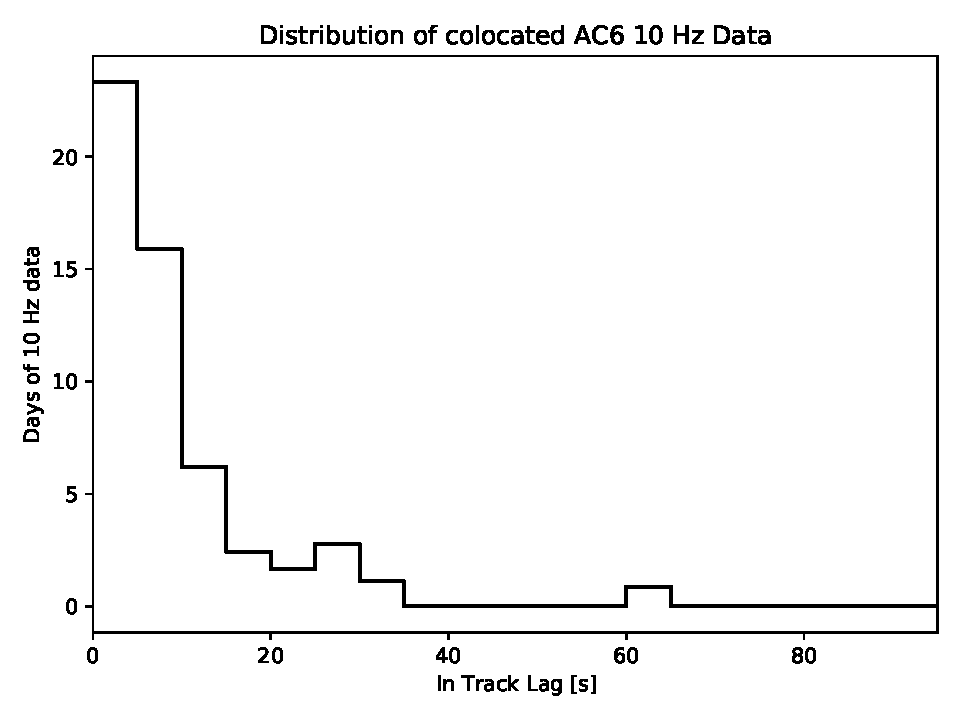
\includegraphics[width=\textwidth]{a_10hz_dist.pdf}
\caption{The distribution of colocated 10 Hz data as a function of in-track lag. Bins are 5 kilometers wide.}
\label{a_10Hz_dist}
\end{figure}

\section{Homeless Words}

Title: Statistical Properties of Curtains--Latitudinally-Narrow and Persistent Electron Precipitation Phenomena

This study leverages AC6, a multi-spacecraft mission, to interpret and understand particle precipitation in a way that is impossible with a single spacecraft.

This study leverages the asymmetry in Earth's magnetic field. The asymmetric magnetic field results in the SAA and the BLC, two very related and unique regions

Particles that impact the atmosphere are lost during that bounce motion. We found curtains in the bounce loss cone, a region in the North Atlantic near and above Iceland.

The bounce loss cone is magnetically connected to the SAA, where Earth's magnetic field is weakest near Earth's surface. A particle observed in the blc in the northern hemisphere will descend below 100 km altitude. At sub-100 km altitudes the particle has a high chance of encountering and scattering with the atmosphere and be lost. 

We found curtain electrons that, when given the chance to execute their cyclical bounce motion, will descend below Earth's surface in the SAA. An electrons can not survive that trip.

Write the paper and ask the question: "What is this paper really about?" Not just curtains, but uncovering something unexpected that has been observed and overlooked for decades.

Are curtains related to aurora? This is a good question---one that is not pertinent here (idea from The Elements of Style p.68).

Here are two parting questions that are not considered here. Why were some curtains shifted slightly? Perhaps it was due to the movement of the magnetic field lines. Also do curtains have a corresponding visual signature on the ground? The answer to this question will show if curtains are related to the aurora.

\bibliography{/home/mike/Dropbox/0_firebird_research/A_presentations/refs}
%\bibliography{"refs"}

\end{document}